\PassOptionsToPackage{unicode=true}{hyperref} % options for packages loaded elsewhere
\PassOptionsToPackage{hyphens}{url}
%
\documentclass[]{article}
\usepackage{lmodern}
\usepackage{amssymb,amsmath}
\usepackage{ifxetex,ifluatex}
\usepackage{fixltx2e} % provides \textsubscript
\ifnum 0\ifxetex 1\fi\ifluatex 1\fi=0 % if pdftex
  \usepackage[T1]{fontenc}
  \usepackage[utf8]{inputenc}
  \usepackage{textcomp} % provides euro and other symbols
\else % if luatex or xelatex
  \usepackage{unicode-math}
  \defaultfontfeatures{Ligatures=TeX,Scale=MatchLowercase}
\fi
% use upquote if available, for straight quotes in verbatim environments
\IfFileExists{upquote.sty}{\usepackage{upquote}}{}
% use microtype if available
\IfFileExists{microtype.sty}{%
\usepackage[]{microtype}
\UseMicrotypeSet[protrusion]{basicmath} % disable protrusion for tt fonts
}{}
\IfFileExists{parskip.sty}{%
\usepackage{parskip}
}{% else
\setlength{\parindent}{0pt}
\setlength{\parskip}{6pt plus 2pt minus 1pt}
}
\usepackage{hyperref}
\hypersetup{
            pdftitle={P8130 Final Project: Predicting Breast Cancer Survival},
            pdfauthor={Guadalupe Antonio Lopez, Gustavo Garcia-Franceschini, Derek Lamb},
            pdfborder={0 0 0},
            breaklinks=true}
\urlstyle{same}  % don't use monospace font for urls
\usepackage[margin=1in]{geometry}
\usepackage{longtable,booktabs}
% Fix footnotes in tables (requires footnote package)
\IfFileExists{footnote.sty}{\usepackage{footnote}\makesavenoteenv{longtable}}{}
\usepackage{graphicx,grffile}
\makeatletter
\def\maxwidth{\ifdim\Gin@nat@width>\linewidth\linewidth\else\Gin@nat@width\fi}
\def\maxheight{\ifdim\Gin@nat@height>\textheight\textheight\else\Gin@nat@height\fi}
\makeatother
% Scale images if necessary, so that they will not overflow the page
% margins by default, and it is still possible to overwrite the defaults
% using explicit options in \includegraphics[width, height, ...]{}
\setkeys{Gin}{width=\maxwidth,height=\maxheight,keepaspectratio}
\setlength{\emergencystretch}{3em}  % prevent overfull lines
\providecommand{\tightlist}{%
  \setlength{\itemsep}{0pt}\setlength{\parskip}{0pt}}
\setcounter{secnumdepth}{0}
% Redefines (sub)paragraphs to behave more like sections
\ifx\paragraph\undefined\else
\let\oldparagraph\paragraph
\renewcommand{\paragraph}[1]{\oldparagraph{#1}\mbox{}}
\fi
\ifx\subparagraph\undefined\else
\let\oldsubparagraph\subparagraph
\renewcommand{\subparagraph}[1]{\oldsubparagraph{#1}\mbox{}}
\fi

% set default figure placement to htbp
\makeatletter
\def\fps@figure{htbp}
\makeatother

\usepackage{setspace}\doublespacing

\title{P8130 Final Project: Predicting Breast Cancer Survival}
\author{Guadalupe Antonio Lopez, Gustavo Garcia-Franceschini, Derek Lamb}
\date{}

\begin{document}
\maketitle

\hypertarget{abstract}{%
\subsection{Abstract}\label{abstract}}

Studies have shown that there are many risk factors combinations for
breast cancer. Fortunately, breast cancer survival rates have increased
and number of deaths have decreased. Nevertheless, it is important to
explore the most significant breast cancer risk factors. To do so, we
used a dataset containing demographic and risk factors information, and
survival status by patients. After cleaning and exploring the data, we
dropped highly correlated variables, combined others, and performed
transformations. We then built the full model, containing an interaction
between estrogen and progesterone status, and selected the best model
using Akaike Information Criterion (AIC). Overall, our final model had a
good ROC-AUC and Brier score values.

\hypertarget{introduction}{%
\subsection{Introduction}\label{introduction}}

Breast cancer occurs due to abnormal cell growths in breast tissue.
Although it is most often found in females, 1 out of every 100 diagnosed
patients in the US is a male. Other breast cancer risk factors include,
increase in age, family history or personal history of breast cancer,
radiation exposure, obesity, alcohol use, among many more. Research
suggests that postmenopausal hormone therapy is a risk factor due the
combination of estrogen and progesterone used to treat signs and
symptoms of menopause.

Additionally, the patient's breast cancer stage is important to consider
when determining the severity of the cancer and how to treat it. The
American Joint Committee on Cancer (AJCC) TNM system is the most common,
and contains clinical and pathologic systems. The pathologic stage is
determined by examining the tissue removed during surgery, while the
clinical stage is based on results of a physical exam, biopsy, and
imaging tests. Nevertheless, both systems are composed of the size of
the tumor, the spread to nearby lymph nodes and/or to distant sites,
their estrogen and/or progesterone receptor status, the grade of the
cancer, and if the cancer makes too much of HER2 protein.

Although, most recently, breast cancer survival rates have increase and
number of deaths decreased, it would be important to explore the risk
factors of breast cancer. For this project, we will investigate the odds
of breast cancer survival given most of the risk factors previously
mentioned.

\hypertarget{methods}{%
\subsection{Methods}\label{methods}}

\hypertarget{data-source}{%
\paragraph{Data source}\label{data-source}}

We obtained a deidentified set containing data on 4024 breast cancer
patients. this dataset contains both demographic information, such as
patient age, race, and marital status; clinical information such as
tumor stage, tumor size, hormone therapies (progesterone and estrogen),
regional node positive, and regional node examined; and outcome
information: the number of months the patient had survived prior to
study conclusion, and their alive/dead status at the end of the study.

\hypertarget{data-cleaning}{%
\paragraph{Data cleaning}\label{data-cleaning}}

We combined the regional node positive and regional node examined
variables into a ``regional node proportion positive'' variable. This
variable, but neither the node positive nor node examined variables were
in the model. Further, we decided to discard the T stage and N stage
variables, as they captured information already contained in the AJCC
6th stage variable. We also excluded the grade variable, as it captured
the same clinical information as the differentiate variable. Due to the
skewness in the distribution of the tumor size, we applied a square root
transformation to that variable (\textbf{Supplemental Figure 1}). We
also added a main\_stage variable, which groups all the stages in
\texttt{6th\_stage} so that ``IIIA'' and ``IIIC'' are under factor level
``III'' for example, and added a white variable that tells us if the
patient is ``White'' or not, essentially grouping ``Black'' and
``Other'' together. Both variables were created in case the reduction of
factor levels makes the fit better.

\hypertarget{model-construction}{%
\paragraph{Model construction}\label{model-construction}}

We decided to use logistic regression model to estimate the risk of
patient death within the followup window. Formally, we assumed that an
for an individual, with probability \emph{p} to die after receiving a
breast cancer diagnosis, the log-odds of \emph{p} was linear, i.e.

\(logit(p_i) = \mathbf{X}\beta+ \epsilon_i\)

Where \textbf{\emph{X}} is the n x p design matrix, and \(\beta\) is a
vector in \(\mathbb{R}^p\).

In addition to the covariates we included the interaction between
\texttt{estrogen\_status} and \texttt{progesterone\_status} given that
we found in our background research that having both ``positive''
increase the chances of breast cancer.

\hypertarget{model-selection}{%
\paragraph{Model selection}\label{model-selection}}

We used a criterion-based method, utilizing Akaike Information Criterion
(AIC) to assess the performance of our models.

\hypertarget{model-validation}{%
\paragraph{Model validation}\label{model-validation}}

We performed 10 cross-validation to assess the performance of our model.
Each observation in a dataset will be in 1 of 10 folds such that it gets
used as training data 9 times, and as test data once. The predictions
are then saved such that each row has an out-of-sample prediction that
can be compared to the real value.

\hypertarget{results}{%
\subsection{Results}\label{results}}

\hypertarget{model-construction-and-selection}{%
\paragraph{Model construction and
selection}\label{model-construction-and-selection}}

We used a logistic model coupled with criterion-based stepwise
regression to determine which variables were useful in predicting the
risk of death in breast cancer patients. The variables that were
identified as important were age, race, marital status, AJCC 6th stage,
differentiate, estrogen status, progesterone status, tumor size, and
regional node positive proportion. Some variables that were not
identified as important by the model were whether the tumor was Stage A
and the interaction between estrogen and progesterone status. For a list
of model coefficients see \textbf{Supplemental Table 1}.

\hypertarget{diagnostics}{%
\paragraph{Diagnostics}\label{diagnostics}}

This is the ROC-AUC for full model on in-sample data, which is a measure
that uses the model's specificity and sensitivity to get a score bounded
by 0 and 1, where 1 is best. This model's ROC-AUC is 0.754.

\includegraphics[width=0.9\linewidth]{written_report_files/figure-latex/roc curve-1}

A brier score was produced to assess the optimal model's performance.
Brier score measures the accuracy of probalistic predictions, where a
score of 0 indicates perfect accuracy. The optimal model's brier score
was 0.112. This suggests that our final model has good probabilistic
prediction accuracy.

\includegraphics[width=0.9\linewidth]{written_report_files/figure-latex/separation plot-1}

\textbf{Figure 2.} Separation plot of model. Values are stripes,
arranged in increasing predicted probability of death. The stripes are
colored yellow if the patient survived, and red if they died. The black
line indicates the predicted probability of death.

This separation plot shows that the model is able to reasonably
effectively distinguish the patients that survived from those that died,
though the low value of the predicted probability across the sample
shows that it gives low probabilities of dying to all subjects.

\hypertarget{model-validation-table-1.}{%
\paragraph{Model validation: Table 1.}\label{model-validation-table-1.}}

This table shows the confusion matrix made from our 10 fold
cross-validation, such that the predicted values are out-of-sample
predictors. Note that cells 1 and 4 (if read from left to right, and
top-down) are individuals for which their status prediction was
correctly predicted, and cells 2 and 4 are individuals for which their
status wasn't correctly predicted.

\begin{longtable}[]{@{}lrr@{}}
\toprule
& Predicted Died & Predicted Survived\tabularnewline
\midrule
\endhead
Actually Died & 3358 & 50\tabularnewline
Actually Survived & 535 & 81\tabularnewline
\bottomrule
\end{longtable}

\hypertarget{model-performance-by-race}{%
\paragraph{Model performance by race}\label{model-performance-by-race}}

Lastly, model performance by race was explored using ROC AUC and Brier
score values. The values by race are presented in the table below.

\begin{longtable}[]{@{}lrr@{}}
\toprule
race & roc\_auc & brier\_score\tabularnewline
\midrule
\endhead
White & 0.760 & 0.109\tabularnewline
Black & 0.704 & 0.171\tabularnewline
Other & 0.650 & 0.088\tabularnewline
\bottomrule
\end{longtable}

\hypertarget{discussion}{%
\subsection{Discussion}\label{discussion}}

We constructed a model to predict the survival of breast cancer
patients, and optimized it using a criterion based-selection approach.
Most of the covariates in the dataset were identified by AIC as being
useful predictors, with the exception of Stage A. Despite the
combination of progesterone (PR+) and estrogen (ER+) receptors in breast
cancer being of note clinically, our model did not find the interaction
term between these variables to be worth including. This suggests that
the adjusted odds ratio for risk of death in ER+/PR+ is 1.

The most significant predictor of death was the regional node positive
proportion variable; an individual with 100\% positive regional nodes
has 3.5 times the odds of death compared with an individual who had no
positive regional nodes. Other highly significant predictors were cancer
stage (specifically whether the patient was IIIC), whether the tumor was
well differentiated (i.e.~healthy cells), hormone receptors on the tumor
(ER+ and PR+), and age.

Our model was effective at classifying patients who survived, but
performed less well at classifying patients who died when using a
\(\hat{p}=0.5\) as the cutoff. The separation plot we constructed
suggests that a lower cutoff, such as 0.35 may be more appropriate, and
further tuning may improve model performance.

Our model was effective at classifying patients who survived, but
performed less well at classifying patients who died when using a
\(\hat{p}=0.5\) as the cutoff. The separation plot we constructed
suggests that a lower cutoff, such as 0.35 may be more appropriate, and
further tuning may improve model performance.

Furthermore, conflicting conclusions occurred while assessing model
performance by race. According to the ROC AUC values, the model
performed better for White patients, then Black patients, then `Other'
race patients. On the contrary, the brier scores by race suggests that
the model most accurately predicted probabilities for `Other' race
patients, followed by White and Black patients.

From our cross-validation confusion matrix, we can see that the model is
very good at correctly predicting that somebody survived, and rarely
predicts the individual died when it didn't. However, the model makes a
lot of errors when trying to predict if the individual survived: more
than 90\% of the total error happens when the model predicts the
individual died, and it actually survived. This reflects the fact that
the model prefers to predict 0 as a result of the \texttt{status}
variable being 0 inflated.

\hypertarget{author-contributions}{%
\subsection{Author Contributions}\label{author-contributions}}

\hypertarget{references}{%
\subsection{References}\label{references}}

American Cancer Society. Breast Cancer Stages. Atlanta, GA: American
Cancer Society, Inc.~Available from:
\href{https://www.cancer.org/cancer/types/breast-cancer/understanding-a-breast-cancer-diagnosis/stages-of-breast-cancer.html\#:~:text=The\%20earliest\%20stage\%20breast\%20cancers,means\%20cancer\%20has\%20spread\%20more.}{https://www.cancer.org/cancer/types/breast-cancer/}

Division of Cancer Prevention and Control, Centers for Disease Control
and Prevention. Breast Cancer in Men. Atlanta, GA: Centers for Disease
Control; 2023 July 25. Available from:
\href{https://www.cdc.gov/cancer/breast/men/index.htm\#:~:text=Breast\%20cancer\%20is\%20most\%20often,is\%20found\%20in\%20a\%20man.\&text=Invasive\%20ductal\%20carcinoma.,parts\%20of\%20the\%20breast\%20tissue.}{https://www.cdc.gov/cancer/breast/men/}

Greenhill B, Ward MD, Sacks A. The separation plot: A new visual method
for evaluating the fit of binary models. American Journal of Political
Science. 2011;55(4):991--1002.
\url{doi:\%5B10.1111/j.1540-5907.2011.00525.x\%5D(https://www.jstor.org/stable/23025132)}

Mayo Clinic. Breast Cancer. Rochester, MN: Mayo Foundation for Medical
Education and Research. Available from:
\href{https://www.mayoclinic.org/diseases-conditions/breast-cancer/symptoms-causes/syc-20352470}{https://www.mayoclinic.org/diseases-conditions/breast-cancer}

Stoica P, Selen Y. Model-order selection: a review of information
criterion rules. IEEE Signal Processing Magazine. 2004;21(4):36--47.
\href{https://ieeexplore.ieee.org/document/1311138}{doi:10.1109/msp.2004.1311138}

Young Survival Coalition. Breast Cancer 101. New York, NY: Young
Survival Coalition. Available from:
\href{https://youngsurvival.org/breast-cancer-101?gad_source=1\&gclid=CjwKCAiAg9urBhB_EiwAgw88mcI-WsyaKEn-nTaWET71dtNVebk2y3qHMeLMjBnxk42z-sE5LMbPPRoCLZYQAvD_BwE}{https://youngsurvival.org/breast-cancer}

\hypertarget{software}{%
\paragraph{Software}\label{software}}

The aforementioned analyses were carried out using R 4.3.1 and RStudio
Version 2023.06.2+561.

\newpage

\hypertarget{supplemental-information}{%
\subsection{Supplemental Information}\label{supplemental-information}}

\hypertarget{table-s1.-model-coefficients}{%
\paragraph{Table S1. Model
Coefficients}\label{table-s1.-model-coefficients}}

\begin{longtable}[]{@{}lrrlrr@{}}
\toprule
\begin{minipage}[b]{0.34\columnwidth}\raggedright
term\strut
\end{minipage} & \begin{minipage}[b]{0.08\columnwidth}\raggedleft
estimate\strut
\end{minipage} & \begin{minipage}[b]{0.09\columnwidth}\raggedleft
std.error\strut
\end{minipage} & \begin{minipage}[b]{0.17\columnwidth}\raggedright
adjusted\_odds\_ratio\strut
\end{minipage} & \begin{minipage}[b]{0.07\columnwidth}\raggedleft
p.value\strut
\end{minipage} & \begin{minipage}[b]{0.09\columnwidth}\raggedleft
statistic\strut
\end{minipage}\tabularnewline
\midrule
\endhead
\begin{minipage}[t]{0.34\columnwidth}\raggedright
age\strut
\end{minipage} & \begin{minipage}[t]{0.08\columnwidth}\raggedleft
0.023\strut
\end{minipage} & \begin{minipage}[t]{0.09\columnwidth}\raggedleft
0.006\strut
\end{minipage} & \begin{minipage}[t]{0.17\columnwidth}\raggedright
1.02 (1.01, 1.03)\strut
\end{minipage} & \begin{minipage}[t]{0.07\columnwidth}\raggedleft
0.000\strut
\end{minipage} & \begin{minipage}[t]{0.09\columnwidth}\raggedleft
4.180\strut
\end{minipage}\tabularnewline
\begin{minipage}[t]{0.34\columnwidth}\raggedright
raceBlack\strut
\end{minipage} & \begin{minipage}[t]{0.08\columnwidth}\raggedleft
0.506\strut
\end{minipage} & \begin{minipage}[t]{0.09\columnwidth}\raggedleft
0.162\strut
\end{minipage} & \begin{minipage}[t]{0.17\columnwidth}\raggedright
1.66 (1.21, 2.28)\strut
\end{minipage} & \begin{minipage}[t]{0.07\columnwidth}\raggedleft
0.002\strut
\end{minipage} & \begin{minipage}[t]{0.09\columnwidth}\raggedleft
3.129\strut
\end{minipage}\tabularnewline
\begin{minipage}[t]{0.34\columnwidth}\raggedright
raceOther\strut
\end{minipage} & \begin{minipage}[t]{0.08\columnwidth}\raggedleft
-0.431\strut
\end{minipage} & \begin{minipage}[t]{0.09\columnwidth}\raggedleft
0.202\strut
\end{minipage} & \begin{minipage}[t]{0.17\columnwidth}\raggedright
0.65 (0.44, 0.97)\strut
\end{minipage} & \begin{minipage}[t]{0.07\columnwidth}\raggedleft
0.033\strut
\end{minipage} & \begin{minipage}[t]{0.09\columnwidth}\raggedleft
-2.132\strut
\end{minipage}\tabularnewline
\begin{minipage}[t]{0.34\columnwidth}\raggedright
marital\_statusDivorced\strut
\end{minipage} & \begin{minipage}[t]{0.08\columnwidth}\raggedleft
0.222\strut
\end{minipage} & \begin{minipage}[t]{0.09\columnwidth}\raggedleft
0.141\strut
\end{minipage} & \begin{minipage}[t]{0.17\columnwidth}\raggedright
1.25 (0.95, 1.65)\strut
\end{minipage} & \begin{minipage}[t]{0.07\columnwidth}\raggedleft
0.115\strut
\end{minipage} & \begin{minipage}[t]{0.09\columnwidth}\raggedleft
1.575\strut
\end{minipage}\tabularnewline
\begin{minipage}[t]{0.34\columnwidth}\raggedright
marital\_statusSingle\strut
\end{minipage} & \begin{minipage}[t]{0.08\columnwidth}\raggedleft
0.153\strut
\end{minipage} & \begin{minipage}[t]{0.09\columnwidth}\raggedleft
0.134\strut
\end{minipage} & \begin{minipage}[t]{0.17\columnwidth}\raggedright
1.17 (0.9, 1.52)\strut
\end{minipage} & \begin{minipage}[t]{0.07\columnwidth}\raggedleft
0.252\strut
\end{minipage} & \begin{minipage}[t]{0.09\columnwidth}\raggedleft
1.146\strut
\end{minipage}\tabularnewline
\begin{minipage}[t]{0.34\columnwidth}\raggedright
marital\_statusWidowed\strut
\end{minipage} & \begin{minipage}[t]{0.08\columnwidth}\raggedleft
0.225\strut
\end{minipage} & \begin{minipage}[t]{0.09\columnwidth}\raggedleft
0.192\strut
\end{minipage} & \begin{minipage}[t]{0.17\columnwidth}\raggedright
1.25 (0.86, 1.83)\strut
\end{minipage} & \begin{minipage}[t]{0.07\columnwidth}\raggedleft
0.242\strut
\end{minipage} & \begin{minipage}[t]{0.09\columnwidth}\raggedleft
1.171\strut
\end{minipage}\tabularnewline
\begin{minipage}[t]{0.34\columnwidth}\raggedright
marital\_statusSeparated\strut
\end{minipage} & \begin{minipage}[t]{0.08\columnwidth}\raggedleft
0.847\strut
\end{minipage} & \begin{minipage}[t]{0.09\columnwidth}\raggedleft
0.366\strut
\end{minipage} & \begin{minipage}[t]{0.17\columnwidth}\raggedright
2.33 (1.14, 4.78)\strut
\end{minipage} & \begin{minipage}[t]{0.07\columnwidth}\raggedleft
0.021\strut
\end{minipage} & \begin{minipage}[t]{0.09\columnwidth}\raggedleft
2.316\strut
\end{minipage}\tabularnewline
\begin{minipage}[t]{0.34\columnwidth}\raggedright
x6th\_stageIIIA\strut
\end{minipage} & \begin{minipage}[t]{0.08\columnwidth}\raggedleft
0.563\strut
\end{minipage} & \begin{minipage}[t]{0.09\columnwidth}\raggedleft
0.163\strut
\end{minipage} & \begin{minipage}[t]{0.17\columnwidth}\raggedright
1.76 (1.28, 2.42)\strut
\end{minipage} & \begin{minipage}[t]{0.07\columnwidth}\raggedleft
0.001\strut
\end{minipage} & \begin{minipage}[t]{0.09\columnwidth}\raggedleft
3.460\strut
\end{minipage}\tabularnewline
\begin{minipage}[t]{0.34\columnwidth}\raggedright
x6th\_stageIIIC\strut
\end{minipage} & \begin{minipage}[t]{0.08\columnwidth}\raggedleft
1.064\strut
\end{minipage} & \begin{minipage}[t]{0.09\columnwidth}\raggedleft
0.193\strut
\end{minipage} & \begin{minipage}[t]{0.17\columnwidth}\raggedright
2.9 (1.98, 4.23)\strut
\end{minipage} & \begin{minipage}[t]{0.07\columnwidth}\raggedleft
0.000\strut
\end{minipage} & \begin{minipage}[t]{0.09\columnwidth}\raggedleft
5.505\strut
\end{minipage}\tabularnewline
\begin{minipage}[t]{0.34\columnwidth}\raggedright
x6th\_stageIIB\strut
\end{minipage} & \begin{minipage}[t]{0.08\columnwidth}\raggedleft
0.413\strut
\end{minipage} & \begin{minipage}[t]{0.09\columnwidth}\raggedleft
0.154\strut
\end{minipage} & \begin{minipage}[t]{0.17\columnwidth}\raggedright
1.51 (1.12, 2.05)\strut
\end{minipage} & \begin{minipage}[t]{0.07\columnwidth}\raggedleft
0.007\strut
\end{minipage} & \begin{minipage}[t]{0.09\columnwidth}\raggedleft
2.676\strut
\end{minipage}\tabularnewline
\begin{minipage}[t]{0.34\columnwidth}\raggedright
x6th\_stageIIIB\strut
\end{minipage} & \begin{minipage}[t]{0.08\columnwidth}\raggedleft
1.141\strut
\end{minipage} & \begin{minipage}[t]{0.09\columnwidth}\raggedleft
0.322\strut
\end{minipage} & \begin{minipage}[t]{0.17\columnwidth}\raggedright
3.13 (1.67, 5.88)\strut
\end{minipage} & \begin{minipage}[t]{0.07\columnwidth}\raggedleft
0.000\strut
\end{minipage} & \begin{minipage}[t]{0.09\columnwidth}\raggedleft
3.546\strut
\end{minipage}\tabularnewline
\begin{minipage}[t]{0.34\columnwidth}\raggedright
differentiateModerately differentiated\strut
\end{minipage} & \begin{minipage}[t]{0.08\columnwidth}\raggedleft
-0.389\strut
\end{minipage} & \begin{minipage}[t]{0.09\columnwidth}\raggedleft
0.104\strut
\end{minipage} & \begin{minipage}[t]{0.17\columnwidth}\raggedright
0.68 (0.55, 0.83)\strut
\end{minipage} & \begin{minipage}[t]{0.07\columnwidth}\raggedleft
0.000\strut
\end{minipage} & \begin{minipage}[t]{0.09\columnwidth}\raggedleft
-3.726\strut
\end{minipage}\tabularnewline
\begin{minipage}[t]{0.34\columnwidth}\raggedright
differentiateWell differentiated\strut
\end{minipage} & \begin{minipage}[t]{0.08\columnwidth}\raggedleft
-0.919\strut
\end{minipage} & \begin{minipage}[t]{0.09\columnwidth}\raggedleft
0.192\strut
\end{minipage} & \begin{minipage}[t]{0.17\columnwidth}\raggedright
0.4 (0.27, 0.58)\strut
\end{minipage} & \begin{minipage}[t]{0.07\columnwidth}\raggedleft
0.000\strut
\end{minipage} & \begin{minipage}[t]{0.09\columnwidth}\raggedleft
-4.776\strut
\end{minipage}\tabularnewline
\begin{minipage}[t]{0.34\columnwidth}\raggedright
differentiateUndifferentiated\strut
\end{minipage} & \begin{minipage}[t]{0.08\columnwidth}\raggedleft
0.961\strut
\end{minipage} & \begin{minipage}[t]{0.09\columnwidth}\raggedleft
0.529\strut
\end{minipage} & \begin{minipage}[t]{0.17\columnwidth}\raggedright
2.61 (0.93, 7.37)\strut
\end{minipage} & \begin{minipage}[t]{0.07\columnwidth}\raggedleft
0.069\strut
\end{minipage} & \begin{minipage}[t]{0.09\columnwidth}\raggedleft
1.816\strut
\end{minipage}\tabularnewline
\begin{minipage}[t]{0.34\columnwidth}\raggedright
estrogen\_statusNegative\strut
\end{minipage} & \begin{minipage}[t]{0.08\columnwidth}\raggedleft
0.738\strut
\end{minipage} & \begin{minipage}[t]{0.09\columnwidth}\raggedleft
0.177\strut
\end{minipage} & \begin{minipage}[t]{0.17\columnwidth}\raggedright
2.09 (1.48, 2.96)\strut
\end{minipage} & \begin{minipage}[t]{0.07\columnwidth}\raggedleft
0.000\strut
\end{minipage} & \begin{minipage}[t]{0.09\columnwidth}\raggedleft
4.169\strut
\end{minipage}\tabularnewline
\begin{minipage}[t]{0.34\columnwidth}\raggedright
progesterone\_statusNegative\strut
\end{minipage} & \begin{minipage}[t]{0.08\columnwidth}\raggedleft
0.571\strut
\end{minipage} & \begin{minipage}[t]{0.09\columnwidth}\raggedleft
0.127\strut
\end{minipage} & \begin{minipage}[t]{0.17\columnwidth}\raggedright
1.77 (1.38, 2.27)\strut
\end{minipage} & \begin{minipage}[t]{0.07\columnwidth}\raggedleft
0.000\strut
\end{minipage} & \begin{minipage}[t]{0.09\columnwidth}\raggedleft
4.485\strut
\end{minipage}\tabularnewline
\begin{minipage}[t]{0.34\columnwidth}\raggedright
root\_tumor\_size\strut
\end{minipage} & \begin{minipage}[t]{0.08\columnwidth}\raggedleft
0.048\strut
\end{minipage} & \begin{minipage}[t]{0.09\columnwidth}\raggedleft
0.031\strut
\end{minipage} & \begin{minipage}[t]{0.17\columnwidth}\raggedright
1.05 (0.99, 1.12)\strut
\end{minipage} & \begin{minipage}[t]{0.07\columnwidth}\raggedleft
0.128\strut
\end{minipage} & \begin{minipage}[t]{0.09\columnwidth}\raggedleft
1.523\strut
\end{minipage}\tabularnewline
\begin{minipage}[t]{0.34\columnwidth}\raggedright
regional\_prop\strut
\end{minipage} & \begin{minipage}[t]{0.08\columnwidth}\raggedleft
1.237\strut
\end{minipage} & \begin{minipage}[t]{0.09\columnwidth}\raggedleft
0.185\strut
\end{minipage} & \begin{minipage}[t]{0.17\columnwidth}\raggedright
3.45 (2.4, 4.95)\strut
\end{minipage} & \begin{minipage}[t]{0.07\columnwidth}\raggedleft
0.000\strut
\end{minipage} & \begin{minipage}[t]{0.09\columnwidth}\raggedleft
6.686\strut
\end{minipage}\tabularnewline
\bottomrule
\end{longtable}

\newpage

\hypertarget{supplemental-figures}{%
\subsubsection{Supplemental figures}\label{supplemental-figures}}

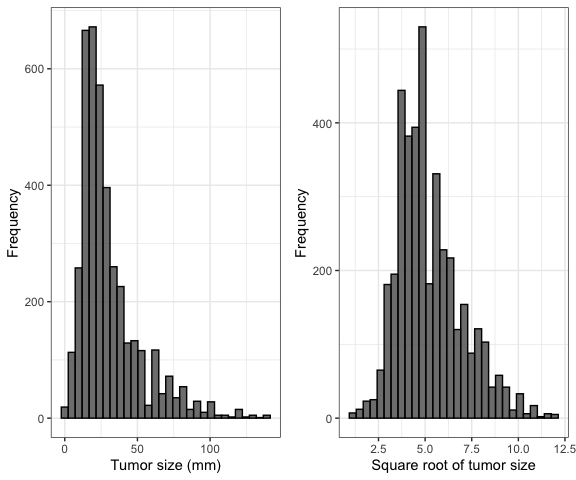
\includegraphics[width=0.9\linewidth]{written_report_files/figure-latex/tumor size transformation hist-1}

\textbf{Figure S1.} Transformation of tumor size variable. (A) Before
transformation. (B) After square root transformation.

\newpage

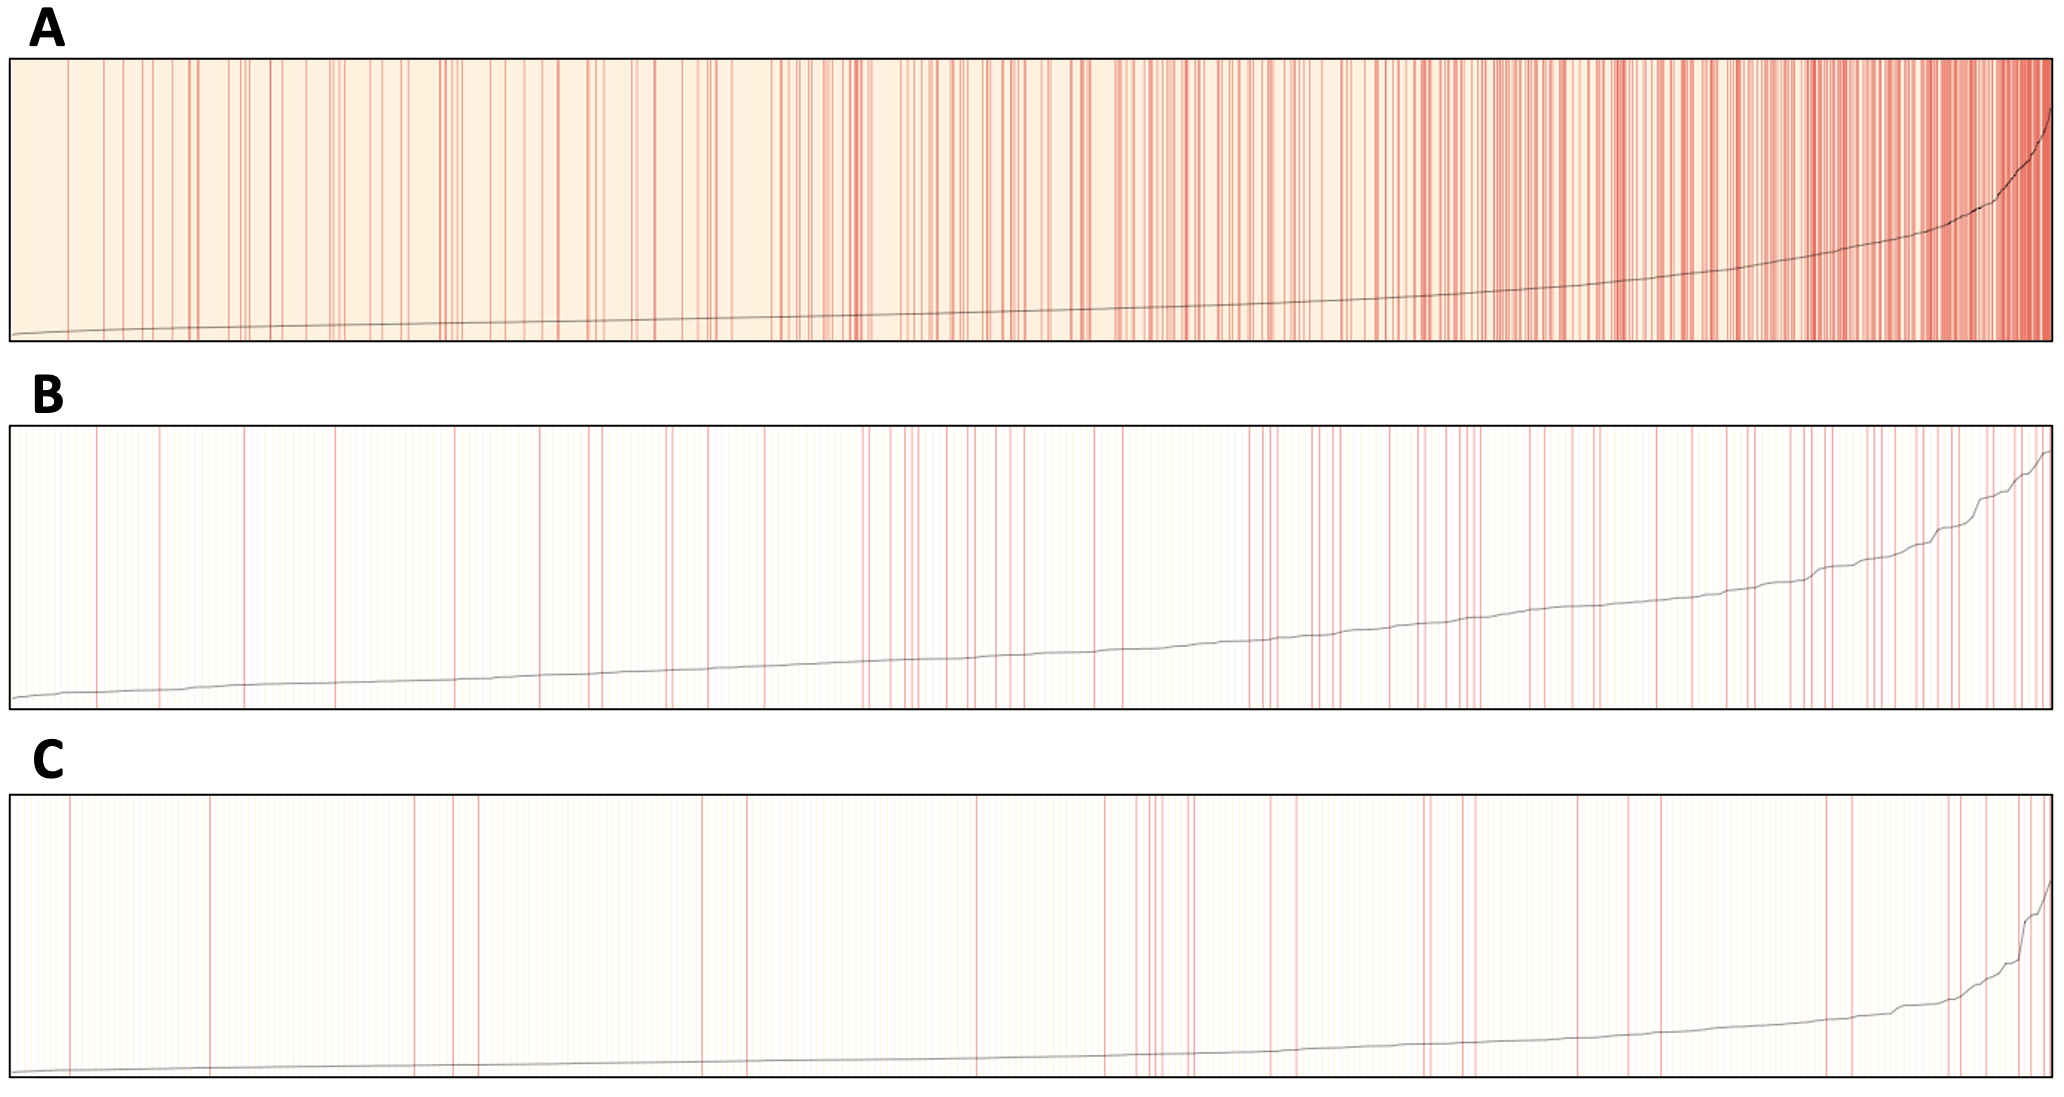
\includegraphics{images/sep_plot_race.png} \textbf{Figure S2.}
Separation plots by race. Values are stripes, arranged in increasing
predicted probability of death in (A) White, (B) Black, and (C) Other
race patients. The stripes are colored yellow if the patient survived,
and red if they died. The black line indicates the predicted probability
of death.

\end{document}
